\section{Schaltgruppenbestimmung}\label{sec:3}
Um die Schaltgruppe zu bestimmen, musste zuerst eine Schaltgruppe gewählt werden und dann über die Anschlussklemmen auf der Sekundärseite des Trafos realisiert werden. Da die Oberspannungsseite bereits als Sternschaltung vorgegeben war, wurde als Schaltgruppe eine \textbf{Yd11} Verschaltung gewählt.\\
Da die Unterspannungswicklungen nur für eine Spannung von \SI{63.5}{\volt} ausgelegt sind, wurden vier Wicklungen pro Strang in Serie geschaltet, wobei der Bezugssinn der Spulen der Primär- und Sekundärseite für den notwendigen Durchflutungsausgleich zu beachten war. Die genaue Verschaltung kann der Abbildung \ref{fig:Verschaltung_Sekundaerseite} entnommen werden.
\begin{figure}[htb]
    \centering
    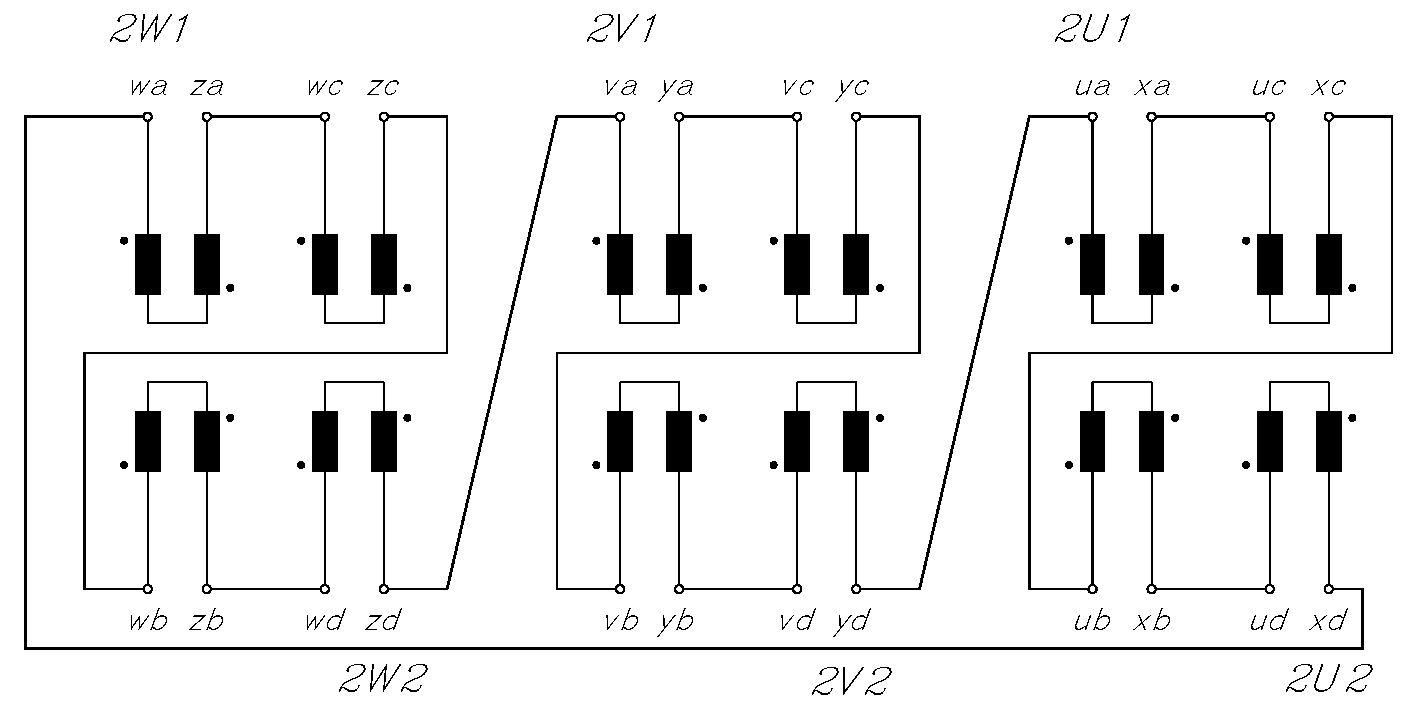
\includegraphics[width=1.0\textwidth, angle=0]{3/images/Schaltgruppe.pdf}
    \caption{Verschaltung der Sekundärwicklungen für eine Yd11 Schaltung}
    \label{fig:Verschaltung_Sekundaerseite}
\end{figure}
Die Schaltgruppenbestimmung dient der Überprüfung der Verschaltung, um sicherzustellen, dass keine Fehler gemacht wurden. Für die Messung muss Primär- und Sekundärseite auf ein gemeinsames Bezugspotential gelegt werden (für Versuchsmessungen zulässig). Dazu wurden die Punkte 1U und 2U verbunden. Die speisende Spannung wurde auf \SI{100}{\volt} begrenzt, wodurch sichergestellt wird, dass die zu messenden Spannungen im zulässigen Messbereich der verwendeten Multimeter zu liegen kommen. Die gemessenen Primär-, Sekundär- und Gegenspannungen für das dreiphasige Zeigerdiagramm (Abb. \ref{fig:schaltgruppe_messung}) sind in der nachstehenden Tabelle \ref{tab:Messwerte_Schaltgruppe} notiert. Die Messschaltung (Schaltgruppe, Messpotential 1U/2U) ist in Abbildung\;\ref{fig:Schaltgruppe_Messschaltung} dargestellt.
\begin{figure}[h!]
    \centering
    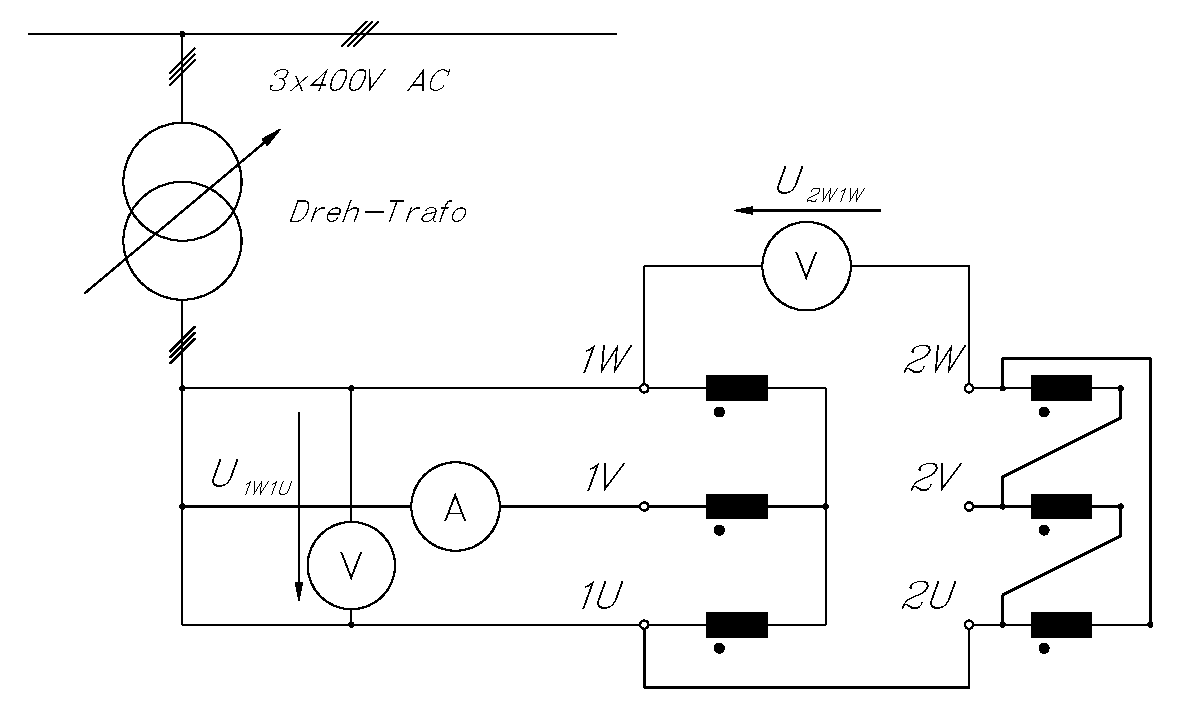
\includegraphics[width=0.75\textwidth, angle =0]{3/images/Schaltgruppe_Messungen.pdf}
    \caption{Messschaltung zur Verifikation der Schaltgruppe \textbf{Yd11}; Messungen der verschiedenen (primär-, sekundärseitigen und gegenseitigen) Spannungen (z.B.: $U_{2W1W}$).}
    \label{fig:Schaltgruppe_Messschaltung}
\end{figure}
\begin{table}[h!]
    \centering
    %\resizebox{\textwidth}{!}
    \caption{Messwerte zur Schaltgruppenbestimmung}
    \label{tab:Messwerte_Schaltgruppe}
\end{table}
Zusätzlich zur Konstruktion des Zeigerdiagramms, wird die Schaltgruppe auch durch die Verhältnisse der Windungszahlen und Spannungen der Ober- und Unterspannungsseite verifiziert.\\
Das Windungsverhältnis ergibt sich aufgrund der Beschaltung der Ober- (Parallelschaltung der 4 Wicklungen) und Unterspannungsseite (Serienschaltung der 4 Wicklungen) lt. Typenschild zu
\begin{equation}
    \Delta_N = \frac{N_{OS}}{N_{US}}=\frac{59}{4\cdot 17}=0,868.
\end{equation}
Daraus lässt sich gemeinsam mit der Schaltgruppe \textbf{Yd} die zu erwartende Spannungsübersetzung zwischen den beiden primär- und sekundärseitigen Aussenleiterspannungen $\Delta_U$ bestimmen:
\begin{equation}
    \Delta_U = \frac{U_{OS}}{U_{US}}=\sqrt{3}\cdot \Delta_N = \sqrt{3}\,\frac{59}{68}=1,503.
\end{equation}
Die gemessene Spannungsübersetzung lässt sich aus dem Verhältnis der beiden gemessenen Aussenleiterspannungen bestimmen (z.B.: zw. W-U):
\begin{equation}
    \Delta_{U,gem} = \frac{U_{1WU}}{U_{2WU}}=\frac{\SI{100}{\volt}}{\SI{66.8}{\volt}}=1,497.
\end{equation}
\input{\currfiledir Yd11}
\input{\currfiledir schaltgruppe}
\clearpage
